%
\index{Logic-tree}
The logic-tree is an integral component of a PSHA input model for the 
OpenQuake-engine since it always contains a logic tree structure 
describing the epistemic uncertainties associated with the construction 
of the seismic source model and a logic-tree used to formally specify 
epistemic uncertainties related to \gls{acr:gsim} models to be used in 
different tectonic regions for the calculation of hazard.

The definition of logic trees in the OpenQuake-engine is based on
the combination of a number of predefined modules each one modelling a 
specific epistemic uncertainty. 
%
Two are the main advantages of this approach. The first and most obvious  
is that the user is not forced to use a predefined logic tree structure and
- instead - can create a tailored logic tree which integrally 
reflects the uncertainties he wants to model. 
%
The second is that the logic tree structure becomes an integral part of  
a PSHA input model definition. The hazard calculations based on this approach
are fully reproducible and do not require pre- or post-processing steps.

This Chapter is dedicated to the description of the basic theory behind 
logic-trees and to the delineation of how logic-trees are implemented 
into the OpenQuake-engine.
%
% ..............................................................................
\section{Introduction}
The use of logic-trees to account for epistemic uncertainties in a 
probabilistic seismic hazard analysis was originally proposed by 
\textcite{kulkarni84}.
%
Nowadays logic-trees are an essential component of a \gls{acr:psha} input
model and represent the formal methodology though which is possible to 
synthesize the results of the estemic uncertainties elicitation process
requested in site-specific seismic hazard analyses \parencite{budnitz1997}
as well as for the creation of state\--of\--the\--art national and 
regional \gls{acr:psha} input models. 

The interpretation of the branches in a logic tree structure, of their 
corresponding weights and of the following results is still the subject 
of an intense scientific debate going on in the literature since 2005 
\parencite{abrahamson2005,mcguire2005,scherbaum2011,musson2012}.
%
However, there is a general agreement on the fact that the branches used to 
describe alternative interpretations (or values of a parameter affected by
epistemic uncertainty) must be mutually exclusive and collectively exhaustive
\parencite{bommer2008}. 
%
This means that  while processing the logic tree, once you choose one option 
in the implementation of a model you automatically exclude the other possible 
interpretations (mutual exclusivity) and that the set of options described 
by the different branches represents the entire group of options admitted 
(collective exhaustiveness). 
%
While the first assumption is relatively easy to accept - although it presumes 
the lack of correlation between the uncertainties in the different branches - 
the second one certainly has implications that are more difficult and delicate 
to go along with since they presumes a comprehensive knowledge of that specific 
model uncertainty, knowledge that cannot be assumed a-priori. 
%
% -------------------------------------------------------------------->>> Figure
\begin{figure}[!ht]
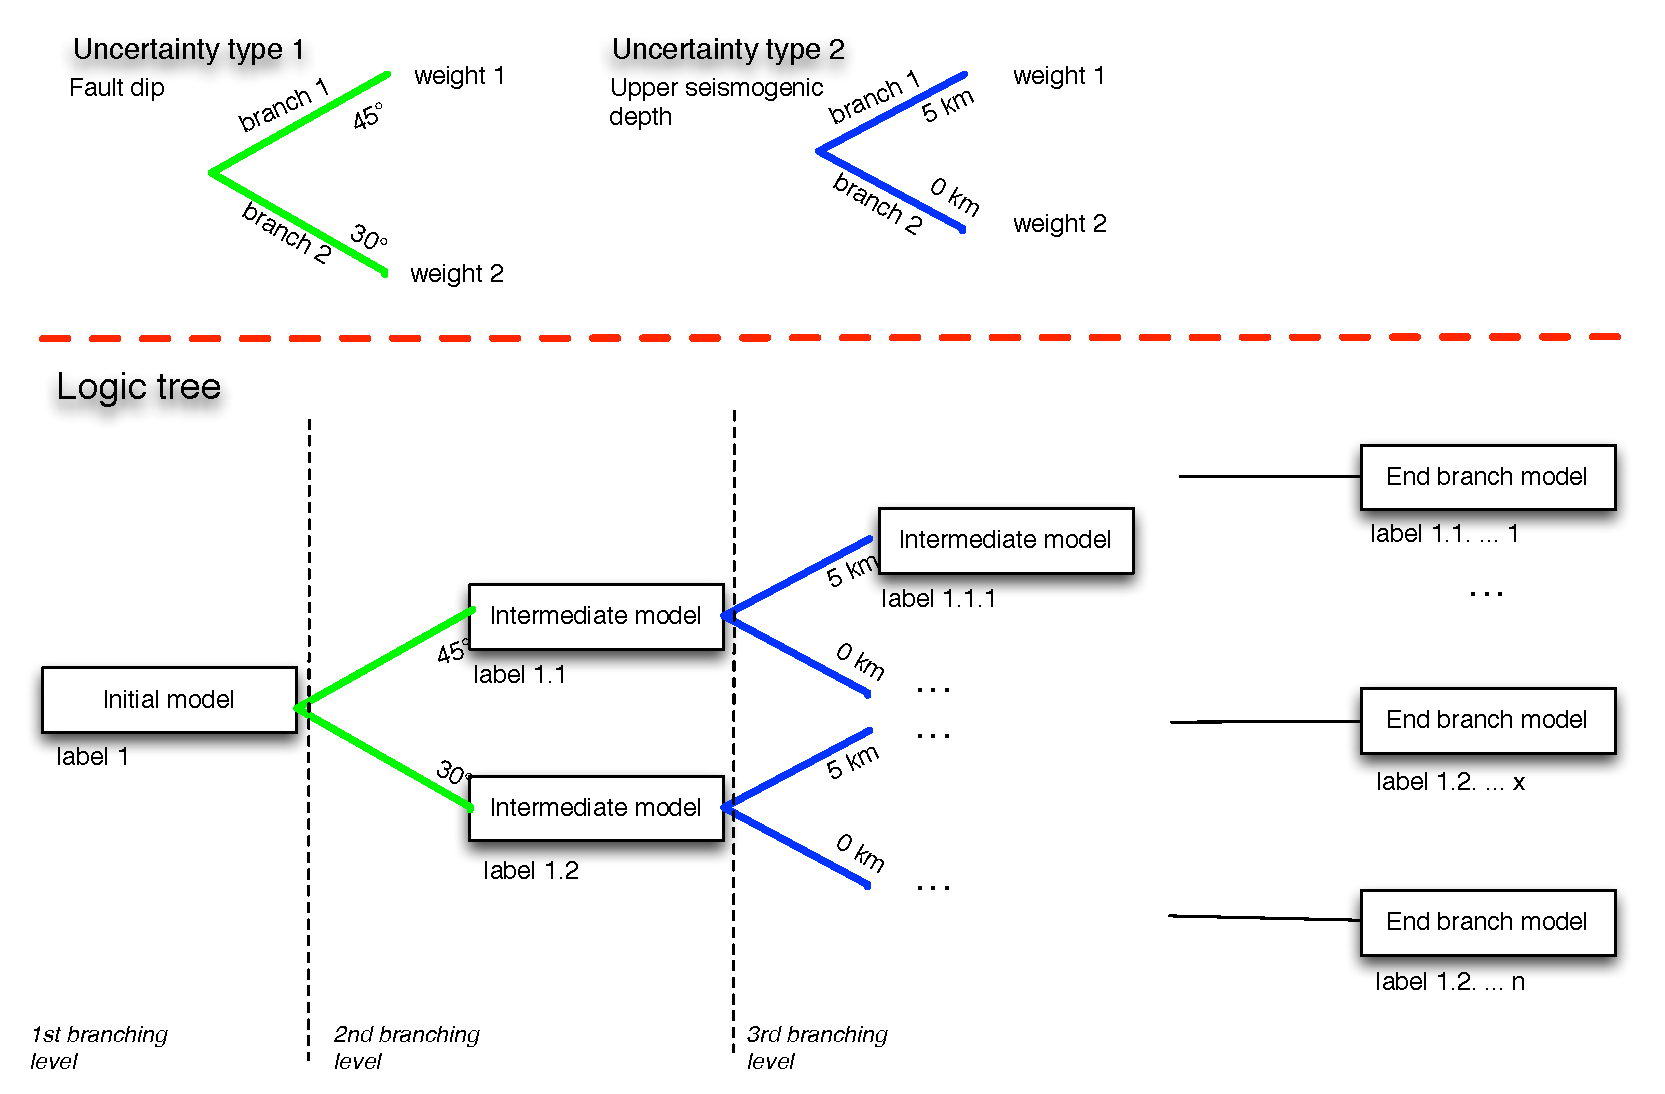
\includegraphics[width=14cm]{./Pictures/lts/logic_tree.pdf}
\caption{An example of modular logic tree structure supported by the
    \gls{acr:oqe}. The upper part of the figure contains two modules, one
    modelling the epistemic uncertainty on the dip angle of a fault, the 
    other modelling the uncertainty on faults upper seismogenic depth.}
\label{fig:logic_tree}
\end{figure}
% --------------------------------------------------------------------<<< Figure
%
% ..............................................................................
\section{The OpenQuake-engine logic-tree structure}
The \gls{acr:oqe}  offers to the user a flexible and modular methodology 
to create customised logic-tree structures. 
%
The logic-trees are defined as a set of linked modules which starting from the 
roots build the logic tree structure until the uppermost branches. The main 
components of this structure are (see for example Figure \ref{fig:logic_tree}):
\begin{itemize}
    \item \emph{branch} \hfill \\
        It is the elemental component of a logic-tree. A tree
        represents one possible interpretation of a model or parameter 
        affected by epistemic uncertainty. It is uniquely defined by a tuple
        consisting of a value and a real number in $[0,1]$ that can be either
        be considered a degree of confidence or a probability.
    \item \emph{branch set} \hfill \\
        A \gls{branchset} is a group of branches where the sum
        of their weights must be equal to one. These branches conceptually 
        represent a complete description of a model/parameter affected by 
        epistemic uncertainty. 
    \item \emph{branching level} \hfill \\
        A branching level defines the position of a 
        branch set within the logic tree structure. The lower is the value of
        the branching level the closer is the branch set to the roots of 
        the tree.
\end{itemize}
A branch set, as well as a \gls{branch}, are defined with a unique 
identifier. 
%
A \gls{branchset} can applied to all the sources included in the initial 
seismic source model, to a subset of sources, to a branch included in a 
branch set occurring before in the logic tree structure or even just to 
a single source. Currently, the rules controlling the application of a 
branch set are the following:
\begin{itemize}
    \item \emph{applyToBranches} \hfill \\
        The current branch set is applied to one 
        or more branches of the previous branching level;
    \item \emph{applyToSources} \hfill \\
        The current branch set is applied to 
        one or more sources in the modelled seismic source model;
    \item \emph{applyToSourceType} \hfill \\
        The current branch set is applied to 
        all the sources of a specific type (e.g. simple fault sources);
    \item \emph{applyToTectonicRegionType} \hfill \\
        The current branch set is applied to all the sources belonging 
        to a selected tectonic region type (e.g. stable continental).
\end{itemize}

The schematic represented in Figure \ref{fig:logic_tree} shows an example of 
the conceptual model adopted to describe a logic tree structure. The
\gls{acr:oqe} provides a set of predefined modules each one modelling a 
specific typology of uncertainty. 
%
% . . . . . . . . . . . . . . . . . . . . . . . . . . . . . . . . . . . . . . .
\subsection{The seismic source model logic tree}
The seismic source model logic tree handles the epistemic uncertainties
related to the definition of geometry, position and seismicity occurrence 
properties of seismic sources. 

The root of the seismic source model logic tree is one (or several) initial 
seismic source model. This means that currently is not possible to create via 
a logic tree a source model by incrementally adding different 
interpretations (e.g. in terms  of geometry) of the sources providing 
contributions to the hazard in a specific site as in the case of the 
recently presented CEUS-SSC model \parencite{ceus2012}. 
%
This functionality will be added in future versions of the software.
%
% . . . . . . . . . . . . . . . . . . . . . . . . . . . . . . . . . . . . . . .
\subsubsection{Supported epistemic uncertainties}
Currently the \gls{acr:oqe} provides a limited set of modules describing a 
specific epistemic uncertainty related to the creation of the seismic source 
model. A short description of each module is provided below.
\begin{itemize}
    \item \emph{Seismic source model} \hfill \\
        It models the uncertainty on the initial seismic source model i.e.
        the set of seismic sources with an assigned geometry and seismicity 
        occurrence properties to be used for the calculation of seismic 
        hazard at the site (or set of sites).
    \item \emph{Relative uncertainty on the maximum magnitude of a double 
            truncated Gutenberg-Richter distribution} \hfill \\ 
        This branch set considers the epistemic uncertainty on the maximum 
        value of magnitude used to define a double truncated Gutenberg-Richter 
        distribution.
    \item \emph{} \hfill \\
        models relative uncertainty on the b-value of double-truncated
        Gutenberg-Richter relationship.
    \item \emph{} \hfill \\ 
        abGRAbsolute
    \item \emph{} \hfill \\ 
        maxMagGRAbsolute
\end{itemize}
%
% . . . . . . . . . . . . . . . . . . . . . . . . . . . . . . . . . . . . . . .
\subsection{The ground-motion model logic tree}
%
\subsubsection{Supported epistemic uncertainties}
Currently the only epistemic uncertainty allowed for the \gls{acr:gsim}
logic-tree.
%
% ..............................................................................
\section{Logic tree processing}
The \gls{acr:oqe} currently provides two distinct ways to process logic-trees.
%
% . . . . . . . . . . . . . . . . . . . . . . . . . . . . . . . . . . . . . . .
\subsection{Full-path enumeration}
Full-path enumeration is the simplest logic-tree processing methodology
implemented. The use of this methodology is possible only when the logic tree
structure is relatively simple i.e. the number of end branches is small. 
%
% . . . . . . . . . . . . . . . . . . . . . . . . . . . . . . . . . . . . . . .
\subsection{Monte Carlo sampling}
Monte Carlo sampling is the processing methodology 
%
% . . . . . . . . . . . . . . . . . . . . . . . . . . . . . . . . . . . . . . .
\subsection{Logic tree pruning/collapsing}
%
% . . . . . . . . . . . . . . . . . . . . . . . . . . . . . . . . . . . . . . .
\subsection{Calculation of mean and percentiles/quantiles}
